\documentclass[a4paper, 12pt]{article}
\usepackage[utf8]{inputenc}
\usepackage[warn]{mathtext}
\usepackage[russian]{babel}
\usepackage[T2]{fontenc}
\usepackage[warn]{mathtext}
\usepackage[justification=centering]{caption}

\usepackage{graphicx}
\graphicspath{ {images/} }
\usepackage{tikz}
\usepackage{pgfplots}

\usepackage{amsmath}
\usepackage{floatflt}
\usepackage[left=20mm, top=20mm, right=20mm, bottom=20mm, footskip=10mm]{geometry}

\usepackage{multicol}
\usepackage{multirow}
\setlength{\columnsep}{2cm}

\usepackage{multicol}
\setlength{\columnsep}{2cm}
\usepackage{hyperref}
\usepackage{wrapfig}

\begin{document}
	
\begin{titlepage}
	\centering
	\vspace{5cm}
	{\scshape\LARGE Московский физико-технический институт \par}
	\vspace{4cm}
	{\scshape\Large Лабораторная работа 5.10.1 \par}
	\vspace{1cm}
	{\huge\bfseries Электронный парамагнитный резонанс \par}
	\vspace{1cm}
	\vfill
\begin{flushright}
	{\large выполнил студент 924 группы ФОПФ}\par
	\vspace{0.3cm}
	{\LARGE Панферов Андрей}
\end{flushright}
	

	\vfill

% Bottom of the page
	Долгопрудный, 2021 г.
\end{titlepage}

\paragraph*{Цель работы:} Исследуется электронный парамагнитный резонанс в молекуле ДФПГ, определяется $g$-фактор электрона, измеряется ширина ЭПР.                                                                              

\section*{Теоретическое введение}
	Энергетический уровень электрона в присутствии магнитного поля с индукцией $B$ расщепляется на подуровня, расстояние между которыми равно 
	\begin{equation}
		\label{eq:dE}
		\Delta E = E_2 - E_1 = 2\mu B.
	\end{equation}
	Здесь $\mu$ -- абсолютная величина проекции магнитного момента на направление поля.
	
	Между этими двумя уровнями возможны переходы. Эти переходы могут возбуждаться внешним высокочастотным электромагнитным полем, если оно имеет нужную частоту и нужное направление.
	
	Резонансное значение частоты определяется из очевидной формулы:
	\begin{equation}
		\label{eq:resonans_omega}
		\hbar \omega_0 = \Delta E.
	\end{equation}

	При переходе с нижнего на верхний уровень энергии электрон поглощает квант электромагнитной энергии, а при обратном переходе такой же квант излучается. Возбуждение электронных резонансных переходов электромагнитным полем, имеющим частоту, определяемую формулой~(\ref{eq:resonans_omega}), носит название электронного парамагнитного резонанса (ЭПР).
	
	В настоящей работе необходимо получить сигнал ЭПР на кристаллическом дифенилпикрилгидразиле (ДФПГ) и определить значение $g$-фактора для электрона. Как известно, связь между магнитным моментом $\mu$ электрона и его механическим моментом $\mathbf{M}$ выражается через гиромагнитное отношение $\gamma$ с помощью формулы
	\begin{equation}
		\label{eq:gyromagnit}
	    \mu = \gamma M.
	\end{equation}
	
	А магнитный момент частицы, измеренный в магнитонах Бора, а механический - в $\hbar$, то их связь можно записать через $g$-фактор:
	\begin{equation}
	    \label{eq:def_g}
	    \frac{\mu}{\mu_\text{Б}} = \frac{M}{\hbar} 
	\end{equation}

	Используя соотношения (\ref{eq:dE})-(\ref{eq:def_g}), нетрудно получить выражение для $g$-фактора через определяемые экспериментально величины:
	\begin{equation}
		\label{eq:g_is}
		\tag{$\star$}
		g = \frac{\hbar \omega_0}{\mu_\text{Б} B}.
	\end{equation}

\newpage
\section{Экспериментальная установка}
	Образец (порошок ДФПГ) в стеклянной ампуле помещяется внутрь катушкииндуктивнсоти входящей в состав колебательного контура. Входящий в состав контура конденсатор состоит из двух платсин, разделенных воздушным зазором, одна из пластин может перемещаться поворотом штока. Колебания в контуре возбуждаются антенной, соединённой с генератором частоты (ВЧ) Г4-116. Амплитуда колебаний поля в катушке индуктивности измеряется по наводимой в петле связи ЭДС индукции. Высокочастотные колебания ЭДС индукции в приёмном контуре детектируются диодом, измеряемая при помощи осциллографа низкочастотная огибающая этого сигнала пропорциональна квадрату амплитуды колебаний поля в катушке.
	\begin{figure}[h!]
	    \centering
			\caption{Схема установки.}
			\label{fig:equip}
			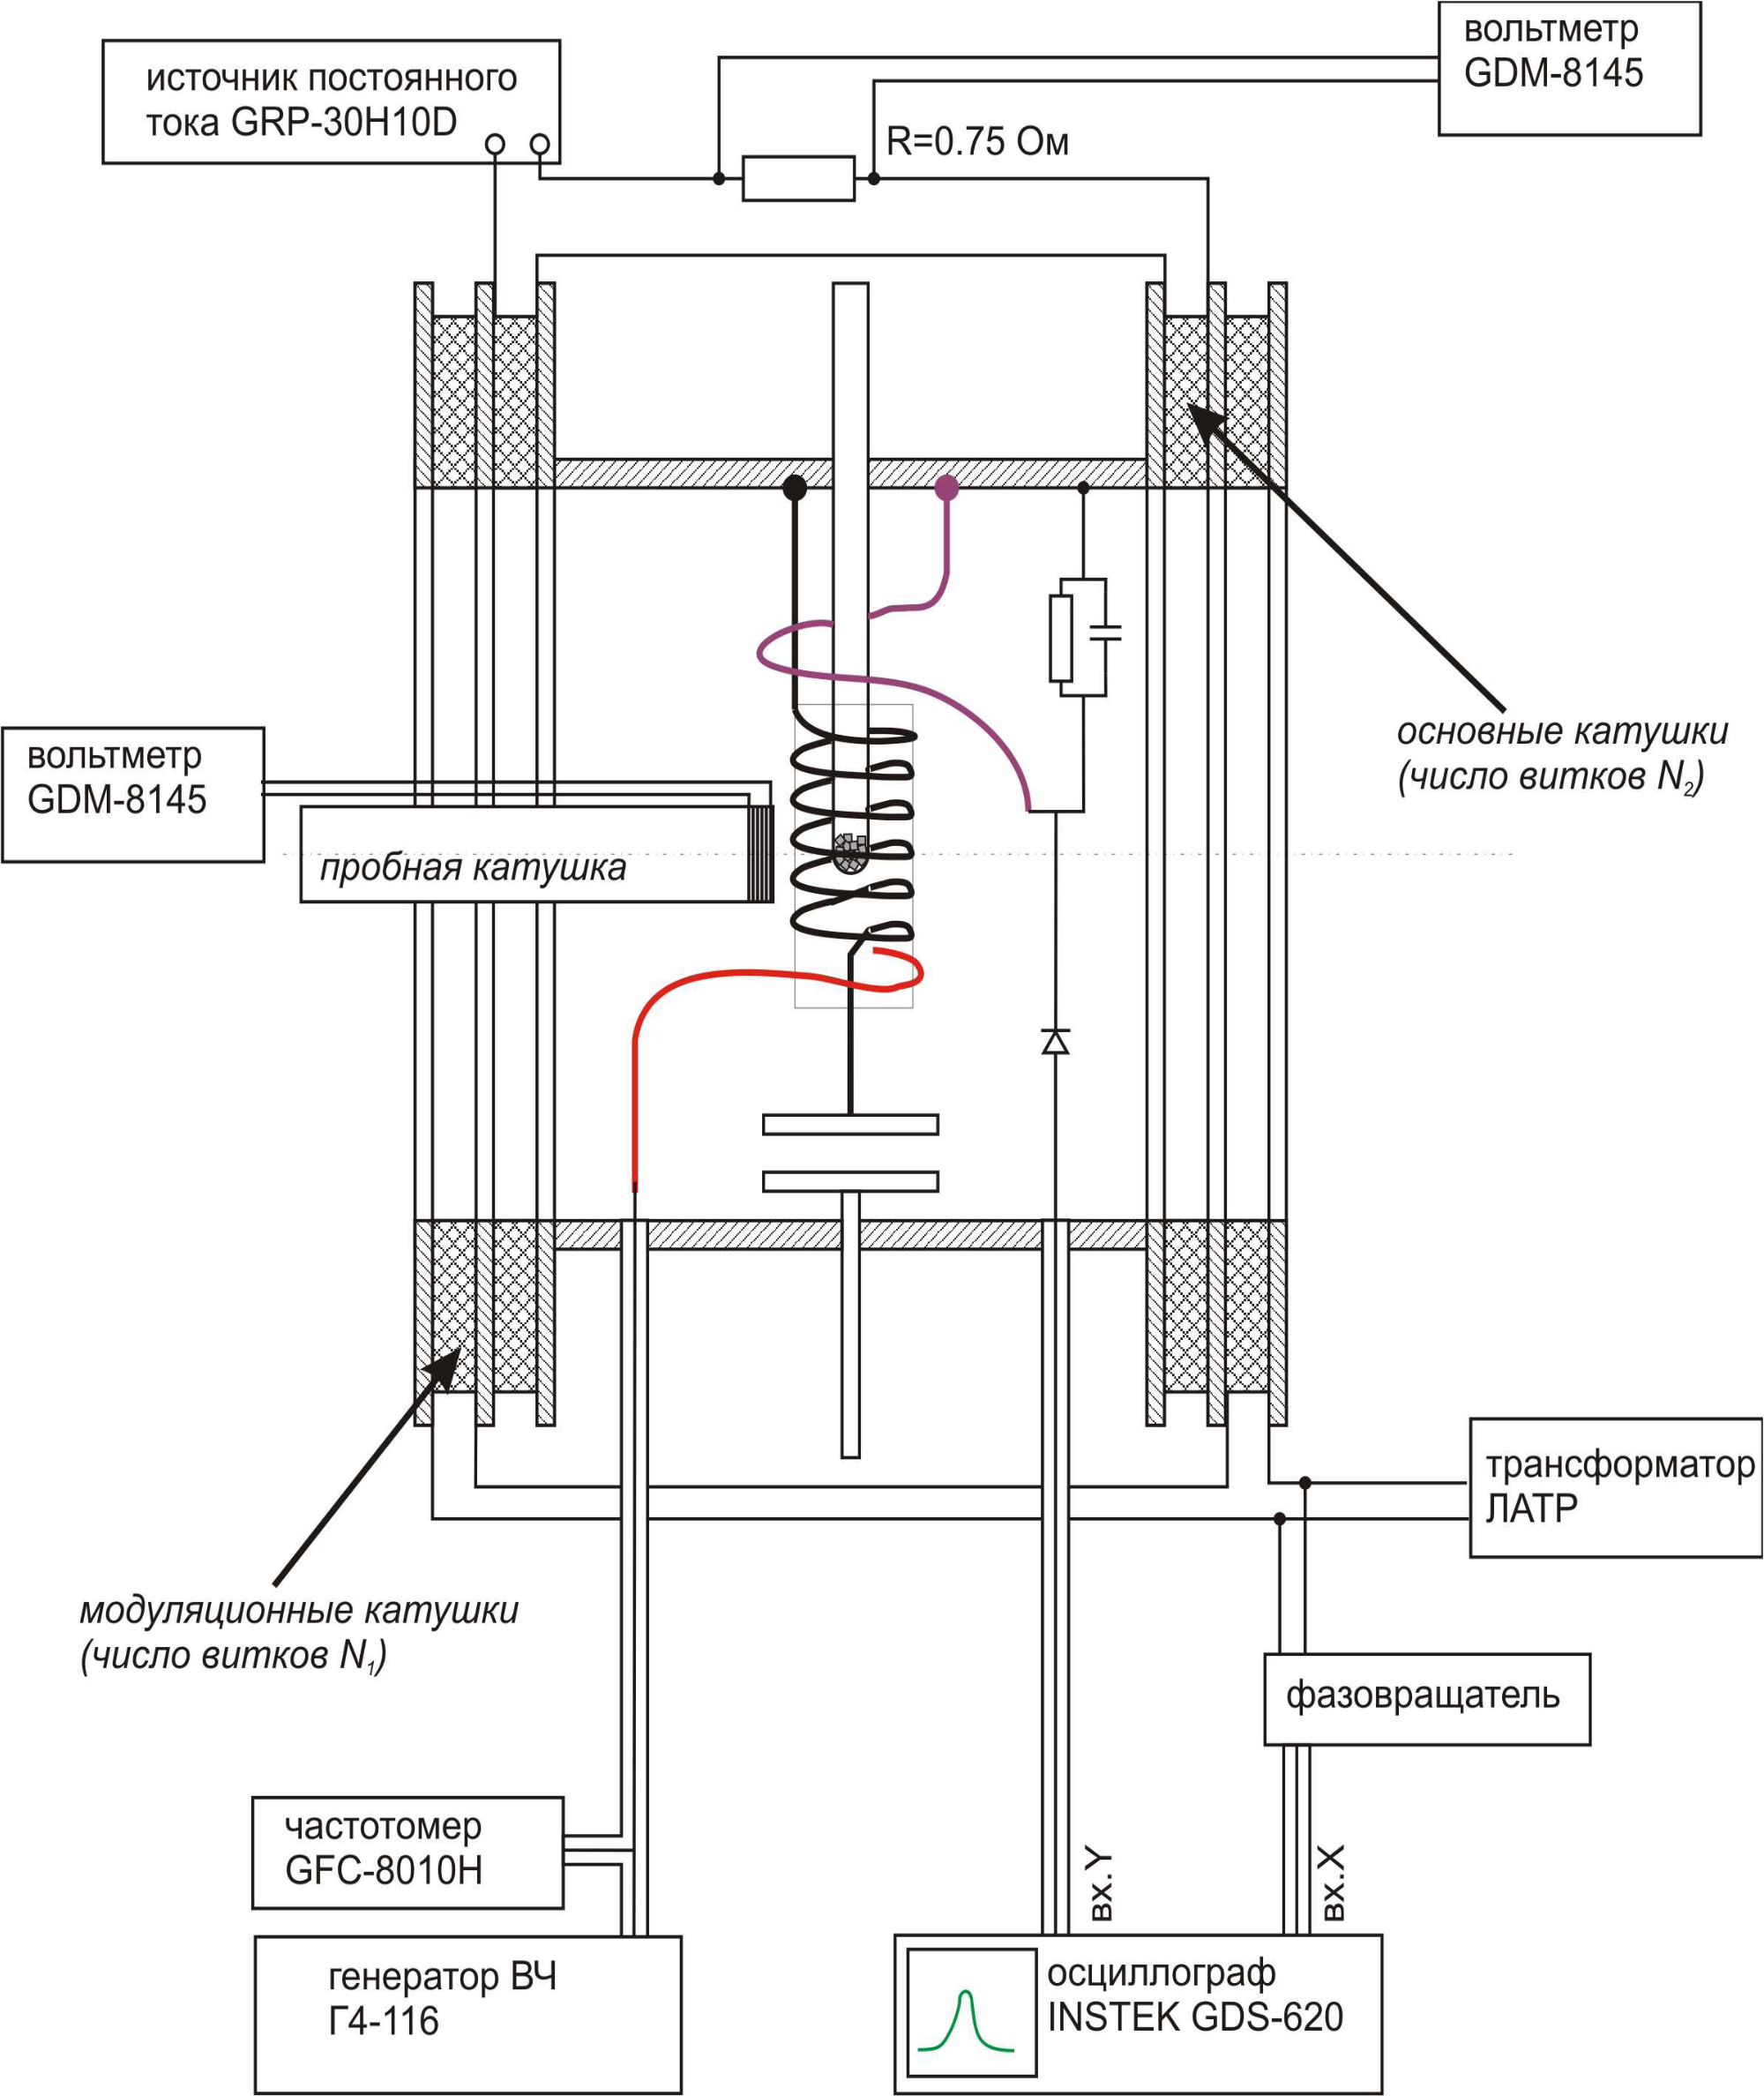
\includegraphics[scale=0.17]{equip.png}
	\end{figure}
	
	Постоянной магнитное поле создаётся пропусканием тока от источника постоянного тока через основные катушки. При этом при помощи вольтметра измеряется падение напряжения на резисторе в цепи основных катушек. Переменное поле небольшой амплитуды создаётся подачей на модуляционные катушки напряжения с регулируемого трансформатора ЛАТР. Для измерения амплитуды колебаний переменного поля используется пробная катушка известной геометрии, подключенная к вольтметру.
	
	
	
	\newpage
	\section*{Ход работы}
	    Запишем параметры катушек в  Таблицу \ref{table:coils}:
	    
	    \begin{table}[h]
	    \label{table:coils}
	    \centering
            \begin{tabular}{|l|l|l|}
            \hline
            \textbf{Катушка} & $N$ & $D$, см \\ \hline \hline
            Основная         & 6700         & $25\pm1$             \\ \hline
            Модуляционная    & 5000         & $30\pm1$             \\ \hline
            Пробная          & 45           & $1.52\pm0.01$             \\ \hline
            \end{tabular}
            \caption{Параметры катушек.}
        \end{table}
        
        \subsection*{Резонанс}
	    
	    
		Настроим генератор на частоту колебательного конутра. Получаем резонансную частоту:
		\begin{equation*}
			f_0 = (164 \pm 1) \ \text{Мгц}.
		\end{equation*}
	
		Подберем величину постоянного магнитного поля в катушках так, чтобы наблюдался сигнал резонанского поглощения. Для этого подадим на катушки достаточное напряжение.
		
		Для более точной настройки и определения ширины линии резонасного поглощения будем наблюдать сигнал в $XY$-режиме. Запишем значение напряжения на резисторе в цепи основных катушек:
		\begin{equation*}
			U_0 = (130 \pm 1) \ \text{мВ}.
		\end{equation*}
		
		\subsection*{Ширина линии поглощения}
	
		Определим ширину линии ЭПР (полуширина на на полувысоте линии резонасного поглощения):
		\begin{equation*}
			\Delta B = \frac{A_{1/2}}{A_{\text{полн}}}B_\text{мод},
		\end{equation*}
		где $A_\text{полн}$ -- полный размах модулирующего поля, $A_{1/2}$ -- ширина кривой на полувысоте, $B_\text{мод}$ -- амплитуда модулирующего поля.
		\begin{equation*}
			\begin{gathered}
				A_\text{полн} = (10 \pm 0.2 ) \ \text{дел}, \ A_{1/2} = (3 \pm 0.2) \ \text{дел} \\
				B_\text{мод} = \sqrt{2} \frac{2\varepsilon}{\pi^2d^2N\nu} = 0.75\pm 0.05 \text{мТл},
			\end{gathered}
		\end{equation*}
		где $\varepsilon$ -- ЭДС индукции при внесении пробной катушки, $N$ -- число витков катушки, $d$ -- диаметр катушки, $\nu$ -- частота модулирующего напряжения (50 Гц).
		
		Имеем:
		\[\boxed{\Delta B = (0.22 \pm 0.02) \ \text{мТл}}.\]
		
		\subsection*{Калибровка основной катушки}
		
		Определим связь между падением напряжения на резисторе в цепи основных катушек и магнитным полем в центре магнита. Поле в центре будем измерять, поднося пробную катушку к основным с двух сторон - спереди и сзади. В качестве значения поля возьмем среднее этих величин. Результаты занесем в Таблицу \ref{table:field}: 
		
		\begin{table}[h]
		\centering
		\label{table:field}
            \begin{tabular}{|c|c|c|c|c|c|}
            \hline
            $V_R$, мВ              & 3.52 & 5.35 & 7.14 & 8.90 & 10.53 \\ \hline
            $V_{\text{перед}}$, мВ & 0.46 & 0.61 & 0.83 & 1.06 & 1.25  \\ \hline
            $V_{\text{зад}}$, мВ   & 0.42 & 0.69 & 0.87 & 1.08 & 1.26  \\ \hline
            $V_{\text{сред}}$, мВ  & 0.44 & 0.65 & 0.85 & 1.07 & 1.255 \\ \hline
            \end{tabular}
        \caption{Калибровочные измерения.}
        \end{table}
        
        Методом наименьших квадратов найдем коэффициент пропорциональности между напряжением на основных катушках и напряжением на пробной катушке:
        \begin{equation*}
            k = 0.120 \pm 0.07
        \end{equation*}
		
		Рассчитав поле, создаваемое основными катушками,
		
		\begin{equation*}
		    B_0 = \frac{4 k U_0}{2\pi\nu N \pi d^2} = (6.1 \pm 0.1) \text{мТл}.
		\end{equation*}
		
		Найдем $g$-фактор электрона:
		
		\begin{equation*}
			g = \frac{hf_0}{\mu_BB_0} = 1.9 \pm 0.1
		\end{equation*}
		

\section*{Вывод}
	В данной работе был исследован ЭПР в молекуле ДФПГ, определяется $g$-фактор электрона $\pmb{g = 1.9 \pm 0.1}$, а также измерена ширина линий ЭПР $\Delta B = 0.22 \pm 0.2~\text{мТл}$. 
	Измеренный $g$-фактор электрона совпадает с табличным значением для свободного электрона: $\pmb{g_{free} = 2,0}$. Это обусловлено тем, что ПР происходит на неспаренных электронах так же, как на свободных.
	


\end{document}